\documentclass[11pt]{article}
\usepackage{amsmath,amssymb,amsthm,graphicx,geometry}
\geometry{margin=1in}

\title{Generalised Monty Hall with Switching Costs:\\
Optimal Stopping, Increasing Marginal Value of Information, and Phase Transitions}
\author{}
\date{}

\newtheorem{theorem}{Theorem}
\newtheorem{proposition}{Proposition}

\begin{document}
\maketitle

% =========================
\begin{abstract}
We study a generalisation of the Monty Hall problem in which an agent faces $K$ doors, $m$ of which contain prizes, and may sequentially acquire information by observing a host reveal non-prize doors at a cost. This transforms the classical puzzle into a deterministic sequential decision problem.  

We derive a closed-form expression for the probability of success under switching after an arbitrary number of reveals and formulate the agent’s decision as an optimal stopping problem. We show that the marginal value of information is strictly increasing in the number of reveals, in contrast to classical models such as Pandora’s box, where marginal value is decreasing.  

This structural property leads to a failure of myopic policies and induces a sharp phase transition in optimal behaviour as a function of information cost. Empirical experiments illustrate these phenomena and confirm theoretical predictions.
\end{abstract}

% =========================
\section{Introduction}

The Monty Hall problem is a canonical example in probabilistic reasoning under partial information. In its classical form, a contestant selects one of three doors, behind one of which lies a prize. The host, who knows the prize location, opens one of the remaining doors that does not contain the prize. The contestant is then given the option to switch. The well-known result is that switching yields a success probability of $2/3$.

This phenomenon arises because the host’s action is constrained by knowledge of the prize location, and therefore redistributes probability mass across remaining doors.

However, the classical setting assumes:
\begin{itemize}
\item a fixed number of doors,
\item a single reveal,
\item zero cost of information.
\end{itemize}

This raises a deeper question:

\begin{center}
\emph{How much information should an agent acquire before making a decision when information is costly?}
\end{center}

We extend the Monty Hall framework to:
\begin{itemize}
\item $K$ doors,
\item $m$ prizes,
\item sequential reveals,
\item cost per reveal.
\end{itemize}

This converts the problem into a structured optimal stopping problem.

\bigskip

\textbf{Core insight:} Information in this setting is \emph{eliminative}, not revelatory. This leads to increasing marginal value of information.

% =========================
\section{Model}

There are $K$ doors, $m$ containing prizes.

\textbf{Initial choice:} The agent selects one door uniformly.

\textbf{Host behaviour:}
\begin{itemize}
\item never opens the chosen door
\item never opens a prize door
\item opens doors sequentially
\end{itemize}

\textbf{Reveals:}
\[
0 \le t \le K - m - 1
\]

\textbf{Costs:}
\[
c_i = c
\]

\textbf{Decision:}
After $t$ reveals, the agent switches uniformly among remaining doors.

\textbf{Objective:}
\[
\mathbb{E}[\text{reward}] - ct
\]

% =========================
\section{Switching Probability}

\begin{theorem}
After $t$ reveals:
\[
P_t = \frac{m(K-1)}{K(K-1-t)}
\]
\end{theorem}

% =========================
\section{Optimal Stopping}

\[
S(t) = \frac{m(K-1)}{K(K-1-t)}, \quad W(t) = S(t) - ct
\]

\begin{theorem}
\[
t^* = \arg\max_t W(t)
\]
\end{theorem}

% =========================
\section{Increasing Marginal Value}

\begin{proposition}
\[
\Delta_t = \frac{m(K-1)}{K(K-2-t)(K-1-t)}
\]
\end{proposition}

\begin{theorem}
$\Delta_t$ is strictly increasing in $t$.
\end{theorem}

\textbf{Interpretation:}
\begin{itemize}
\item Early reveals → low value
\item Late reveals → high value
\end{itemize}

This is the central structural property.

% =========================
\section{Failure of Myopic Policies}

Myopic rule:
\[
\Delta_t \ge c
\]

\textbf{Observation:}
\begin{itemize}
\item Early $\Delta_t$ small → reject
\item Late $\Delta_t$ large → accept
\end{itemize}

Thus:
\begin{itemize}
\item myopic policy stops at $t=0$
\item optimal policy continues to $t=K-2$
\end{itemize}

% =========================
\section{Phase Transition}

There exists $c^*(K)$ such that:

\[
t^* =
\begin{cases}
0 & c > c^* \\
K-2 & c < c^*
\end{cases}
\]

\[
c^*(K) \approx \frac{1}{K}
\]

\textbf{Key property:}
\begin{itemize}
\item no gradual transition
\item abrupt jump in optimal policy
\end{itemize}

% =========================
\section{Experiments}

We simulate for $K=50, m=1$.

\subsection{Experiment 1: $S(t)$ vs $t$}

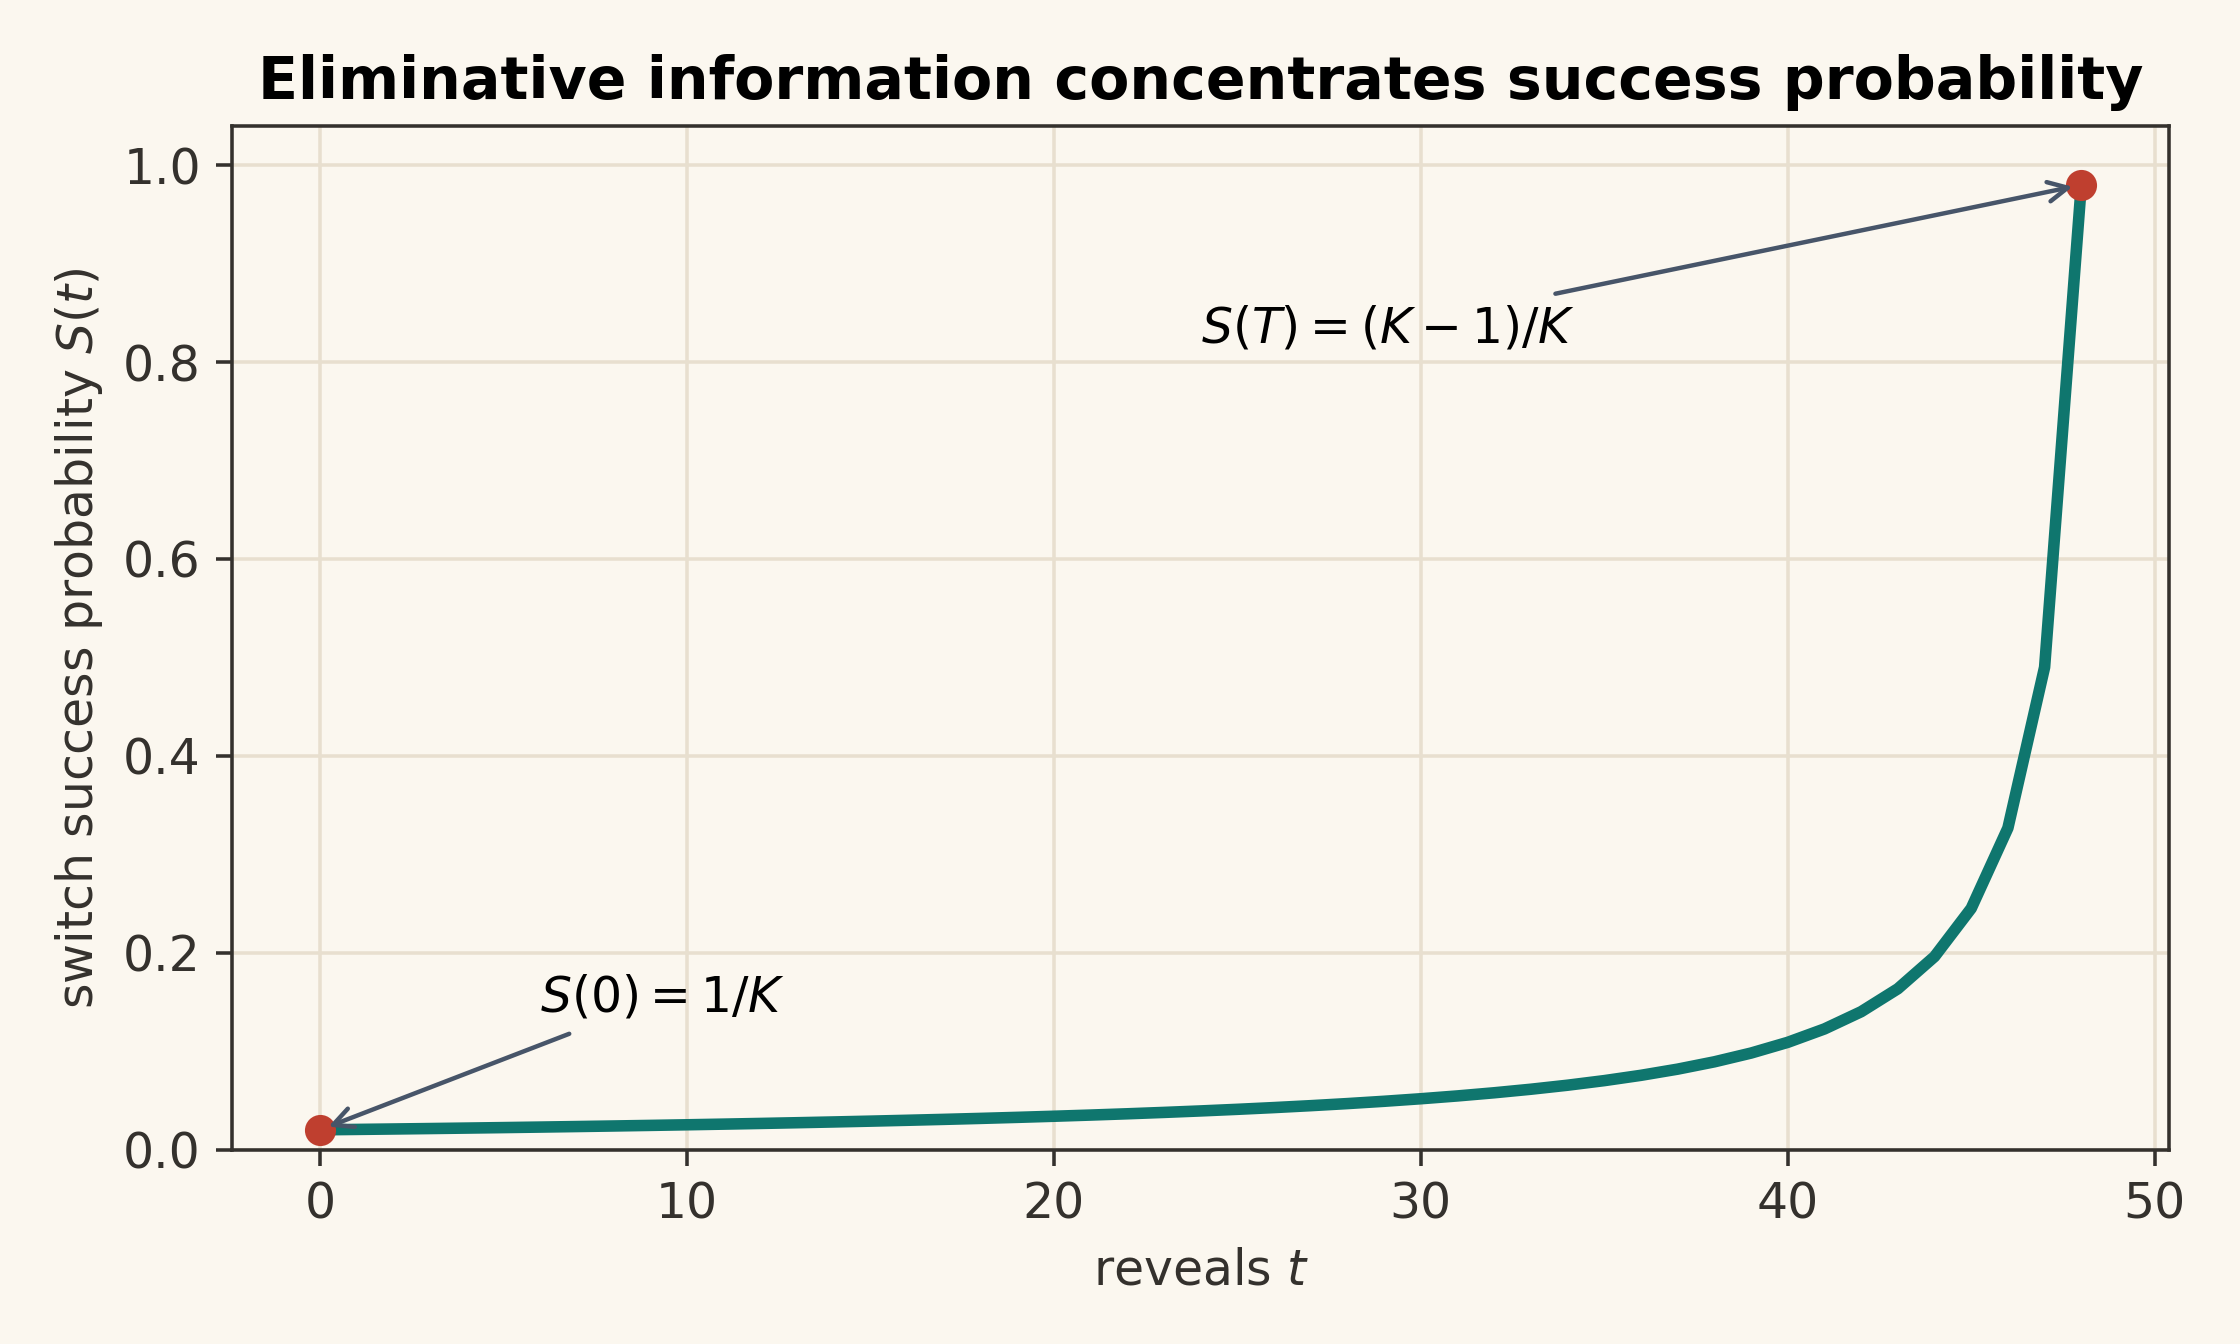
\includegraphics[width=0.85\textwidth]{fig_S.png}

\textbf{Observation:}
\begin{itemize}
\item flat initially
\item sharp rise near $t=K-2$
\end{itemize}

\textbf{Interpretation:}
This explains why early reveals are low-value and late reveals dominate.

% =========================
\subsection{Experiment 2: $W(t)$ vs $t$}

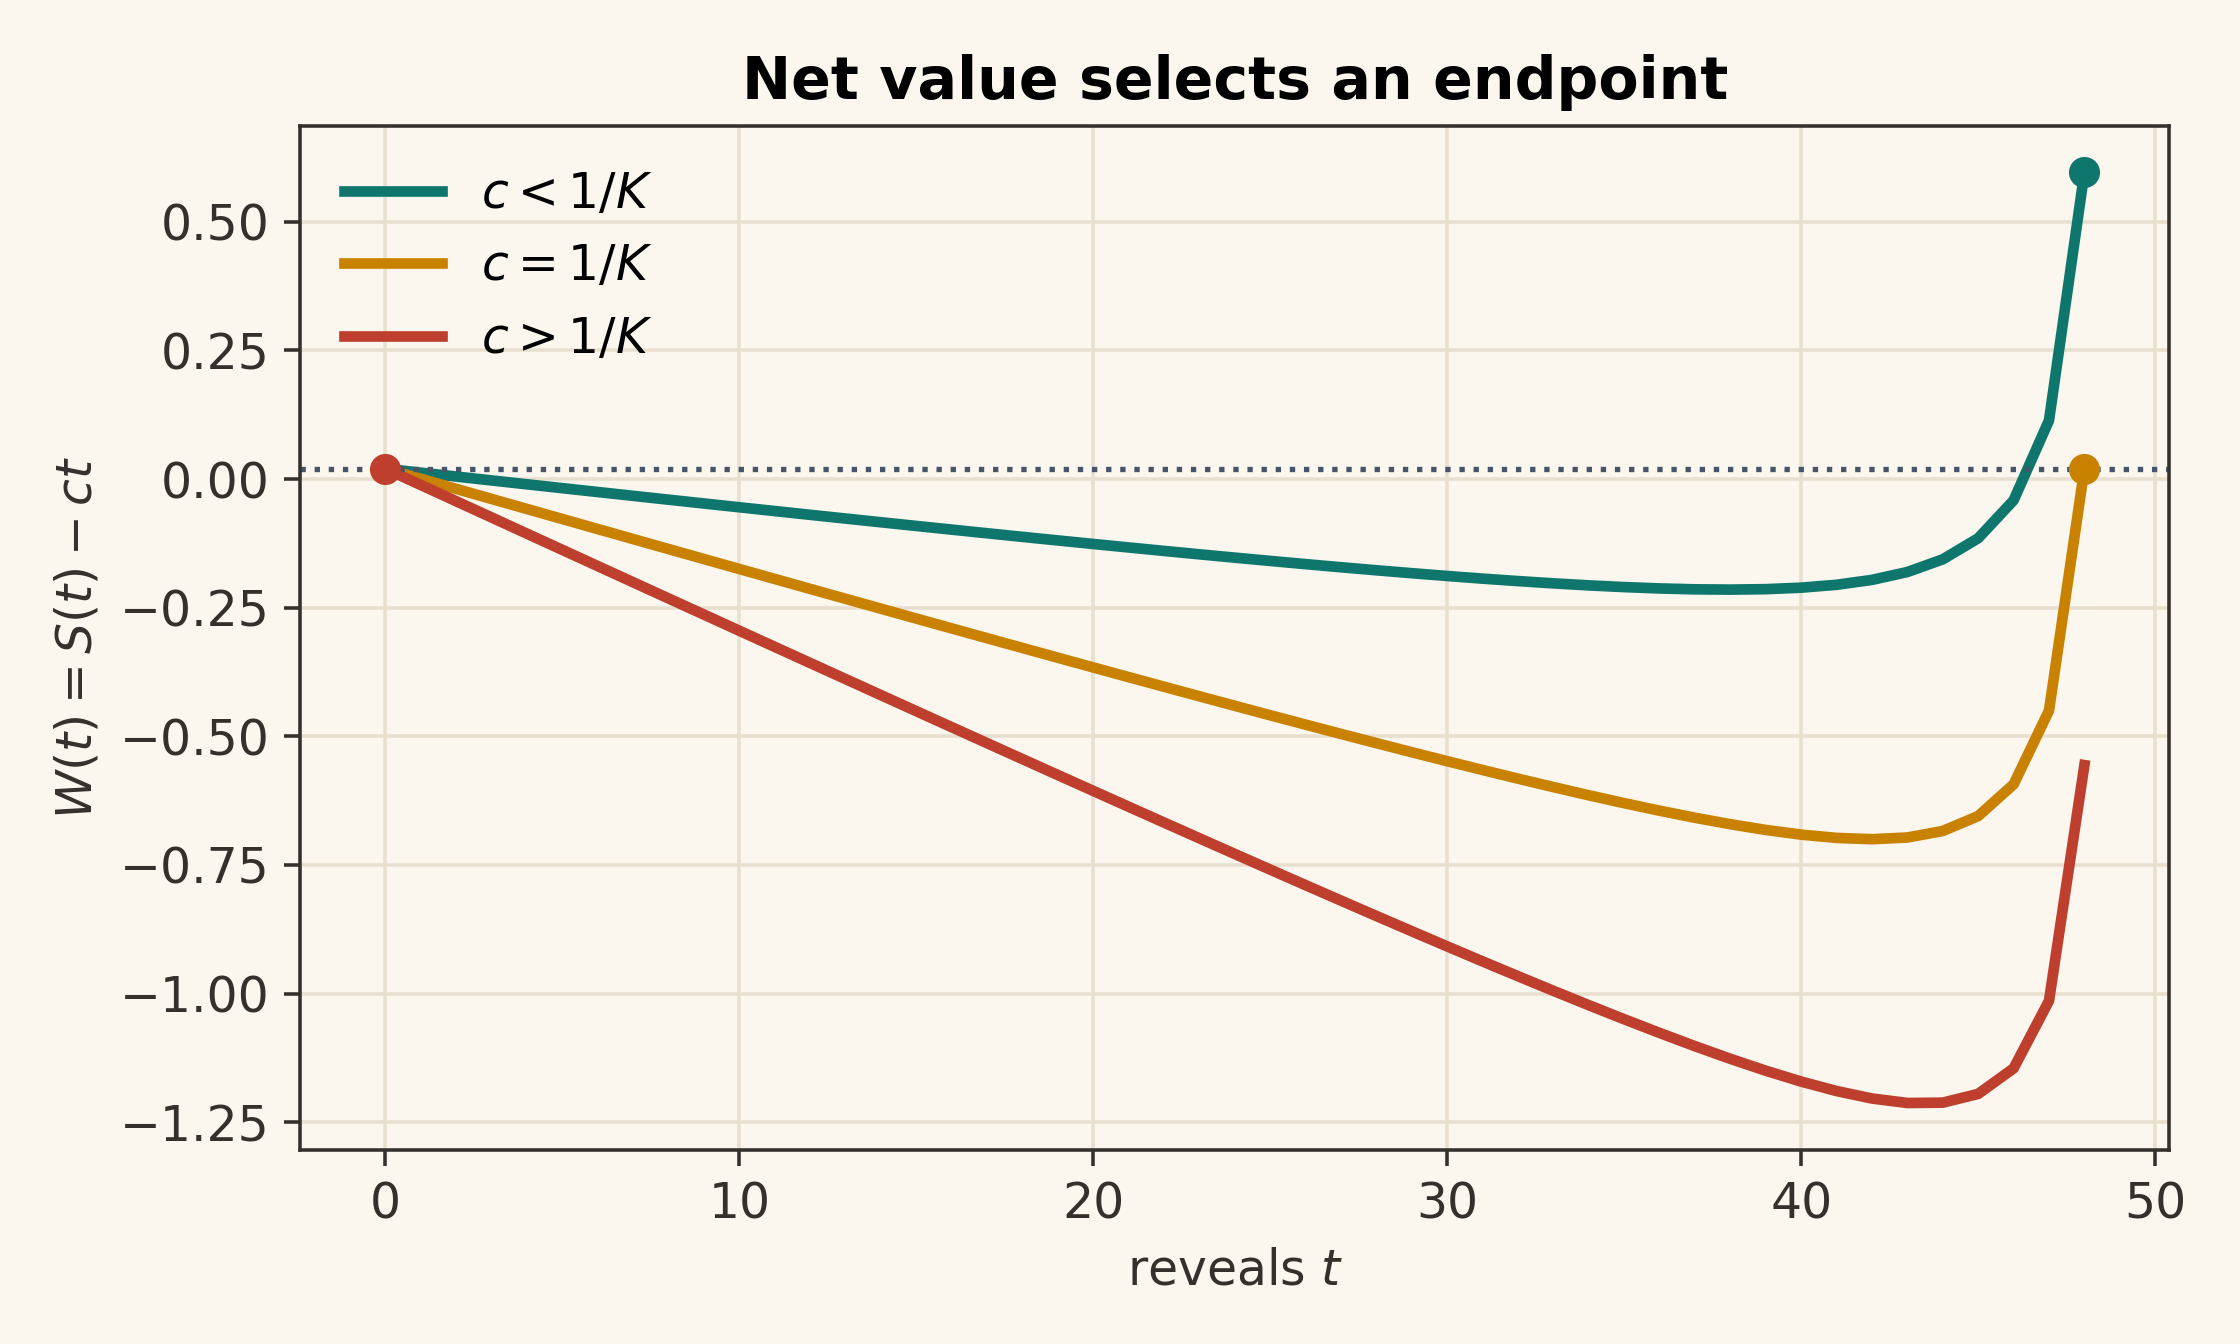
\includegraphics[width=0.85\textwidth]{fig_W.png}

\textbf{Observation:}
\begin{itemize}
\item non-monotonic
\item early negative slope
\item late dominance
\end{itemize}

\textbf{Interpretation:}
Cost competes with convex reward, producing non-trivial optimum.

% =========================
\subsection{Experiment 3: $t^*$ vs $c$}

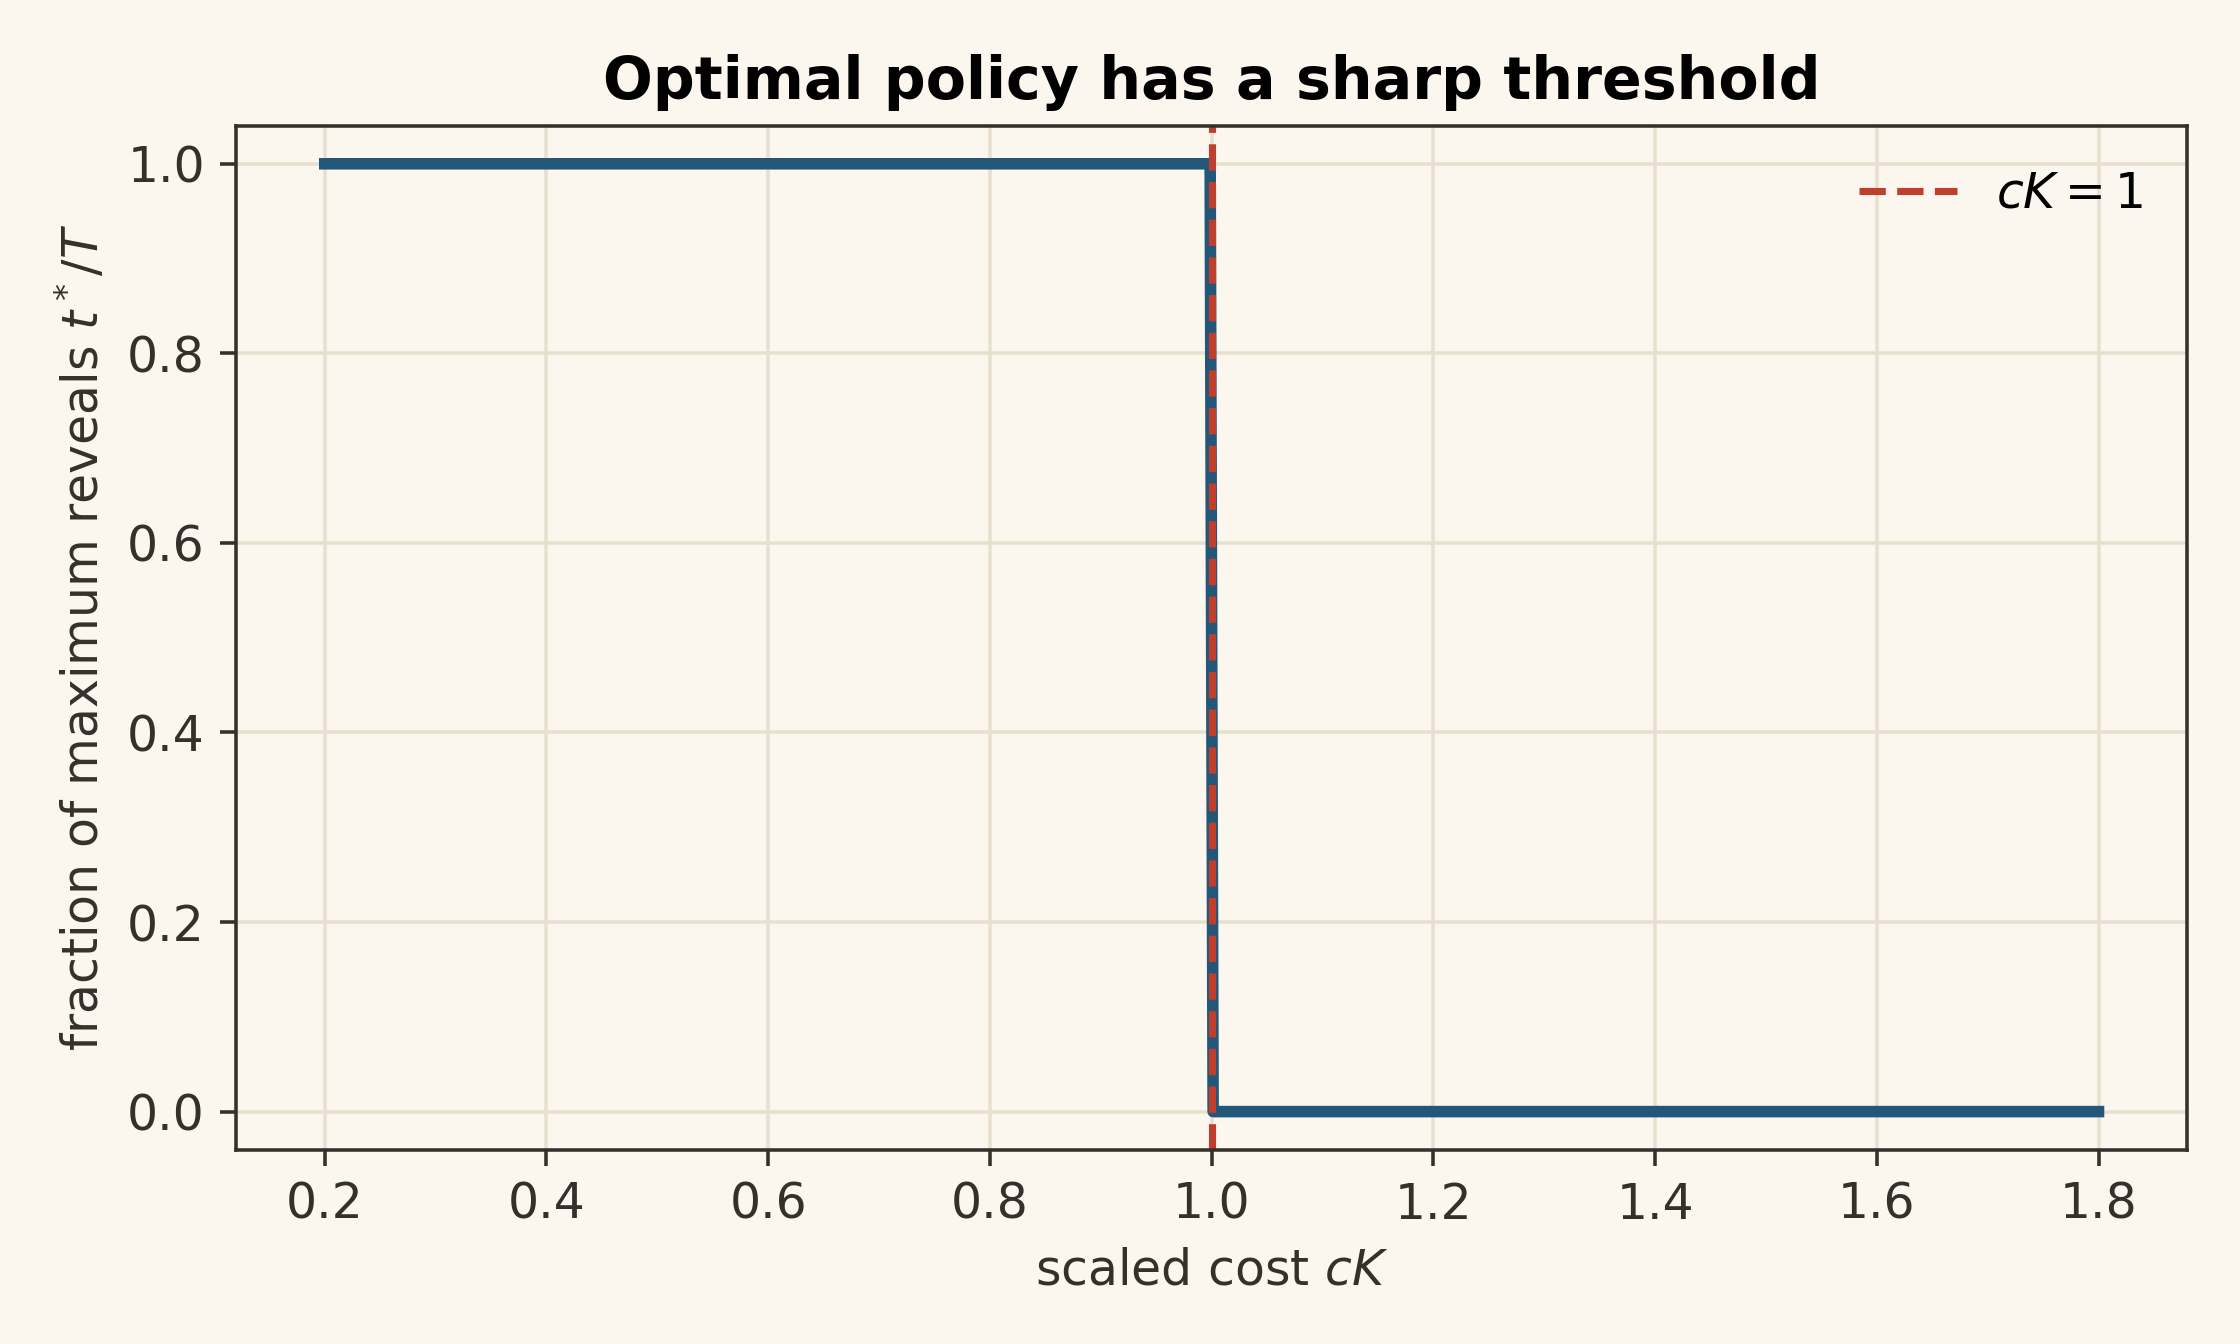
\includegraphics[width=0.85\textwidth]{fig_tstar.png}

\textbf{Observation:}
\begin{itemize}
\item sharp discontinuity
\item no smooth transition
\end{itemize}

\textbf{Interpretation:}
This is the phase transition: optimal policy jumps from no reveals to full reveals.

% =========================
\section{Comparison to Pandora’s Box}

\begin{tabular}{lcc}
\hline
Property & Pandora & This work \\
\hline
Information & value & elimination \\
Marginal value & decreasing & increasing \\
Policy & index & non-myopic \\
\hline
\end{tabular}

\textbf{Key distinction:}
Pandora relies on diminishing returns — violated here.

% =========================
\section{Conclusion}

We show that:

\begin{itemize}
\item information value increases
\item greedy policies fail
\item optimal strategy exhibits phase transition
\end{itemize}

This provides a clean counterexample in information acquisition theory.

% =========================
\section{Future Work}

\begin{itemize}
\item stochastic hosts
\item Bayesian priors
\item adversarial settings
\item bandit formulations
\end{itemize}

\end{document}
